\section{Simulating Serverless Edge Computing Systems}
We choose FaaS-Sim\cite{faas-sim-github} as our simulation framework.
FaaS-Sim is is a state of the art serverless computing simulation built on SimPy, %todo cite simpy
a discrete even simulation tool.
From an architectural basis, FaaS-Sim is built to mimic a serverless framework similar to OpenFaaS.
FaaS-Sim is built on top of a simulated Kubernetes infrastructure, meaning that it too has the notion of containers, container images, resource requirements, scaling, and scheduling.
Because FaaS-Sim is built with evaluating serverless edge computing in mind, it also includes support for representing a wide array of node hardware with heterogeneous capabilities and performance.
\begin{table}[]
\begin{tabular}{lcccc}
\hline
\textbf{Bin}        & \textbf{LOW}  & \textbf{MED} & \textbf{HIGH} & \textbf{VERY HIGH} \\ \hline
CPU Cores (logical) & 1 - 2         & 4 - 8        & 16 - 32       & \textgreater 32    \\
Memory              & 1 to 2        & 4 - 8        & 9 - 32        & \textgreater 32    \\
CPU Frequency (GHz) & \textless 1.5 & 1.6 - 2.2    & \textless 3.5 & \textgreater 3.5   \\ \hline
\end{tabular}
\caption{Resource binning used for performance categorization and prediction with Ether devices by Raith, Rausch and Dustdar\cite{philipp-da}}
\label{tab:ether_bins}
\end{table}

\begin{table}[]
\begin{tabular}{lrrrrr}
\hline
\textbf{\begin{tabular}[c]{@{}l@{}}Device\\ Name\end{tabular}} & \textbf{\begin{tabular}[c]{@{}r@{}}CPU\\ Arch\end{tabular}} & \textbf{\begin{tabular}[c]{@{}r@{}}CPU\\ Cores\end{tabular}} & \textbf{\begin{tabular}[c]{@{}r@{}}CPU\\ Freq\end{tabular}} & \textbf{\begin{tabular}[c]{@{}r@{}}Memory\\ GiB\end{tabular}} & \textbf{GPU/AI Accel}   \\ \hline
RPi3                                                           & arm32v7                                                     & 4                                                            & LOW                                                         & 1                                                             & -                       \\
RPi4                                                           & arm32v7                                                     & 4                                                            & MED                                                         & 1                                                             & -                       \\
RockPi                                                         & aarch64                                                     & 6                                                            & MED                                                         & 4                                                             & -                       \\
Coral                                                          & aarch64                                                     & 4                                                            & MED                                                         & 1                                                             & Google TPU co-processor \\
Intel NUC                                                            & x86\_64                                                     & 4                                                            & MED                                                         & 16                                                            & -                       \\
Jetson Xavier NX                                                             & aarch64                                                     & 6                                                            & LOW                                                         & 8                                                             & 384-core Volta          \\
Jetson Nano                                                           & aarch64                                                     & 4                                                            & LOW                                                         & 4                                                             & 128-core Maxwell        \\
Jetson TX2                                                           & aarch64                                                     & 4                                                            & LOW                                                         & 8                                                             & 256-core Pascal        \\
Intel Xeon                                                           & x86\_64                                                     & 4                                                            & HIGH                                                        & 8                                                             & -                       \\
Intel Xeon + GPU                                                      & x86\_64                                                     & 4                                                            & HIGH                                                        & 8                                                             & Nvidia Turing GPU       \\ \hline
\end{tabular}
\caption{Table showing the simulated devices available in FaaS-Sim/Ether. CPU frequency bin sizes are shown in Table \ref{tab:ether_bins}}
\label{tab:ether_devices}
\end{table}



Table \ref{tab:ether_devices} shows an overview of the hardware devices our simulated clusters are comprised of.

Scheduling in FaaS-Sim is based on the work of Rausch et al.\cite{skippy}, and uses an exact re-implementation of the Kubernetes scheduler, making it an exact representation of that component's behaviour in real-life.
Scaling works like it does in OpenFaaS, meaning that functions can be scaled either via \gls{hpa} or via OpenFaaS' trace driven approach.
Of course, the system also allows for custom and experimental scaling mechanisms to be integrated.
For some of our evaluations we do integrate such custom scaling behaviour, or more precisely the option to disable scaling at will, and to use a fixed replica counts instead, to remove this variability from certain evaluations if necessary.

For the purposes of this work we extended FaaS-Sim to feature a second, parallel, and completely separate scaling and scheduling system.
As the placement of load balancers in serverless edge computing systems is one of the core aspects of this work, this second scaling and scheduling system is tasked only with determining the amount and location of load balancers.
All other parts of the serverless system are scaled and scheduled using the first system.
The two systems are entirely separate from each other, with the exception that they share the node resources containers are placed on.

Being a serverless computing simulator, FaaS-Sim also includes the concept of functions.
Functions are, just like they are in OpenFaaS, an application running in a containerized fashion on the Kubernetes cluster, with a number of replicas determined by the scaler.
To simulate function invocations, particularly the \gls{fet} component, FaaS-Sim relies on pre-defined statistical distributions to sample from.
For every request these distributions are sampled to determine the \gls{fet} of the invocation.
FaaS-Sim supports the use of different distributions for each type of device present in the system, which allows FaaS-Sim to build on trace data from real-world deployments to make its own simulation more accurate.
For our evaluations, we build on the work done in this area by Raith, Rausch and Dustdar\cite{philipp-da}.
FaaS-Sim also includes a model for performance degradation based on the computational capacity of the nodes, meaning that given a high enough request load single nodes become unable to handle all of them in reasonable time.
To provide some variability, we simulate a cluster that has three serverless functions deployed: \textit{Resnet50-Inference}, \textit{Mobilenet-Inference}, and \textit{Speech-Inference}


These functions all represent \gls{ai} inference workloads as these the cornerstone to enabling edge intelligence\cite{rauschEdgeIntelligenceConvergence2019} through serverless edge computing.
They are also an example of network bound workloads, usually featuring fast request processing, and are impacted significantly potential network congestion or long latencies.
\begin{figure}
    \centering
    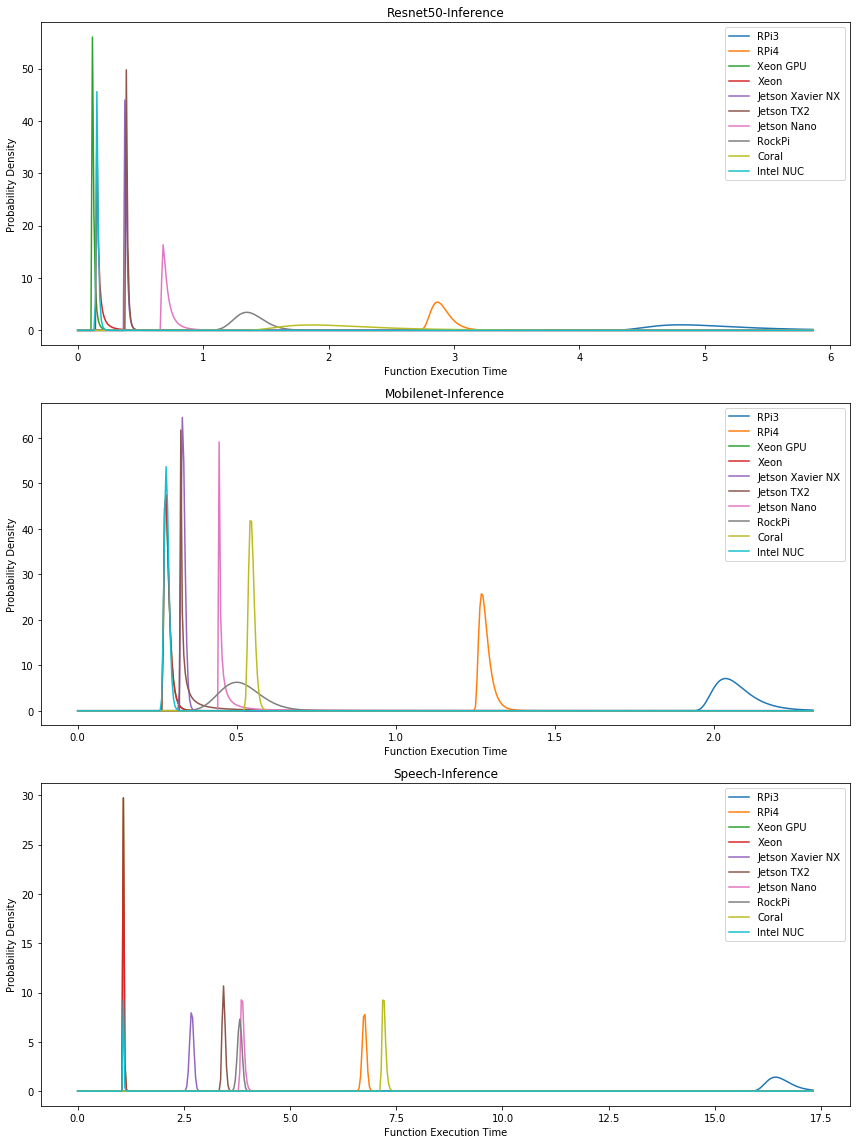
\includegraphics[width=\linewidth]{graphics/graphs/devices_fets.png}
    \caption{Probability density functions of the \glspl{fet} of the different devices we simulate}
    \label{fig:devices_fets}
\end{figure}

Figure \ref{fig:devices_fets}
shows the \gls{fet} distributions for these functions on the hardware outlined in Table \ref{tab:ether_devices}.

Because FaaS-Sim originally only supported response time evaluations due to \gls{fet}, we extend it to also include the network time incurred from request transfers.
To enable this functionality, we introduce the notion of clients explicitly.
They are represented via nodes in the underlying network topology, just like the serverless cluster's nodes are.
Each request is dispatched from a client, sent to the nearest running load balancer instance, on to the function instance the load balancer selects, and back the same way.

The load pattern clients exhibit in FaaS-Sim can be fully controlled.
Generally, clients follow a predefined request pattern, either individually or globally, but absolutely any pattern required can be implemented.
This allows the simulation of differently active clients, differently active regions, and request patterns that change depending on system parameters.

To extract data for later analysis, FaaS-Sim features fine-grained and extensible trace-logging of all requests and system events.